\ifdefined\THESIS
    \chapter{\uppercase{Location Prediction}}
\else
    \section{Location Prediction}
\fi

Based on the questions we answered in the previous section, we have enough
information to build a system for location prediction, which we call
FriendlyLocation.
%
Since the location prediction system will be run on a large number of users,
it must be fast and scalable.
%
In Chapter~\ref{chap:eval} we will evaluate this system using five-fold cross
validation.
%
In this chapter we will use the numbers from one of the five folds to make
the descriptions more concrete.

\section{Edge Length Prediction}

We need to separate the best contacts, who are likely to be nearby, from
bad contacts who are likely to be far away.
%
The factors that we investigated in the previous section indicate when someone
is likely to be nearby, but they don't guarantee it.
%
There are pairs of users who are reciprocal friends with a small number of
followers, a high local friend ratio, have conversations, and still live on
opposite sides of the globe.
%
Another problem with this data is that some of these factors are correlated
with each other; users with lots of followers tend to have a low friend contact
ratio.
%
Finally, distant accounts like celebrities may be useless for determining which
city a person is from, but they might still suggest the user's home continent.

In \cite{backstrom2010find}, the authors present a model of the relationship
between distance and friendship that treats all of the edges the same.
%
We can improve the accuracy of this model by weighting some edges more strongly
than others.
%
We have several pieces of information, and want to map it to a single, extremely
noisy value: the distance to a contact.
%
This could be looked at as a classification problem where you want to classify
edges as local or non-local, but the problem is there is a smooth continuum
from local to non-local, and semi-local friends can be useful for location
prediction.
%
As a result, we model this as a regression problem.
%
Since most of the input features are correlated and either binary or non-linear,
linear regression is unlikely to work well.
%
In addition, the data is dense and low-dimensional, so Support Vector Machines
do not work well.
%
We chose to use a decision tree regressor based on the CART algorithm
(classification and regression trees) to distinguish the best edges from the
worst.
%
A decision tree regressor works similar to the well-known decision tree
classifier, except that it produces real numbers as output instead of discrete
classes.
%
During training, the training data is recursively split based on the input
variable with the most predictive power to build a binary tree.
%
Each of the internal nodes of this tree have a cutoff for one of the input
variables, and the leaves of the tree have a predicted value.
%
\jam{Does this need a better explanation? Can we assume people know decision
trees?}

The regression tree was trained on several of the features from the previous
section that are correlated with users living near each other:
\begin{itemize}
\item the type of contact
\item if the target mentioned the contact
\item if the contact mentioned the target
\item if the contact had a protected account
\item the contact's follower and friend count
\item the PLE of the contact's location
\item the contact's local friend ratio
\end{itemize}
%
Since the distances between users varied by several orders of magnitude, we
trained the regressor to predict the log of the distance.
%
The tree regressor was configured to not split leafs with fewer than 1000 data
points to prevent over-fitting.
%
The top three levels of a decision tree are shown in Figure~\ref{fig:TreeTop}.
%
The predictor does not do a great job of predicting the actual distance to a
contact; there's simply too much noise.
%
However, it does do an excellent job of separating the closest pairs of users
from the most distant pairs as we will show in the next section.

\begin{figure}[tbh]
\centering
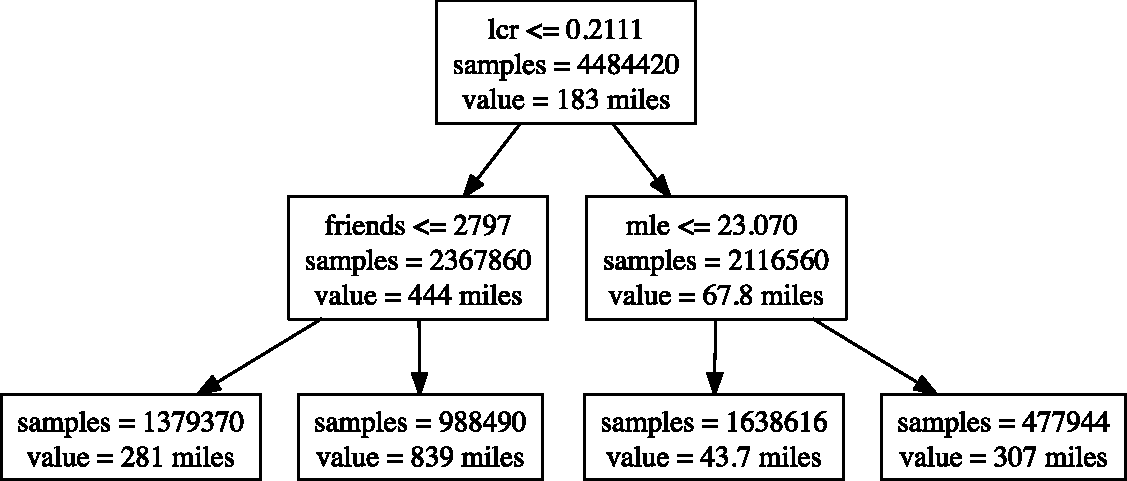
\includegraphics[width=\linewidth]{figures/tree_top.pdf}
\caption{
    The top three levels of the decision tree. This decision tree will predict a
    distance of 839 miles for a contact with a local contact ratio of .2 and
    2800 friends. It will predict a much-closer distance of 43.7 miles for a
    user with a local contact ratio of .5 and a predicted location error of 10
    miles.
}
\label{fig:TreeTop}
\end{figure}

\section{Model}
\label{sec:model}

In the previous sections, we looked at the probability that a contact lives a
certain distance from a given user.
%
In this section, we build a model for the probability that a user, who we refer
to as the target user, lives at a specific location given the approximate
location of his contacts.
%
We will extend the model presented in \cite{backstrom2010find}.
%
Here's how they described their curve for the probability of friendship as a
function of distance:
\begin{quote}
To generate this curve, we aggregate over all individuals, computing the
distance between all $8.1 \times 10^{12}$ pairs of individuals with known
addresses.
We then bucket by intervals of 0.1 miles to compute the total number of pairs
and the number of pairs for which an edge is present, plotting the ratio. It
turns out that we can get a good fit to a curve of the form $a(b+x)^{-c}$.
The exponent very close to $c=-1$ suggests that, at medium to long-range
distances, the probability of friendship is roughly inversely proportional to
distance.
\end{quote}

There are several differences between what they did and what we are doing.
%
First, the data we have is from around the world, so we consider distances up
to 10,000 miles apart instead of stopping at 1,000 miles.
%
The data is a lot noisier in the 1,000--10,000 mile range because of the
distribution of land and oceans on the earth.
%
Next, their dataset had street addresses for approximately 2.9 million
Americans, and they used the friendships between users with street addresses to
do the calculation.
%
Since our geolocated users rarely have connections with other geolocated users
we use the geocoded locations of their contacts, which are less accurate than
street addresses since the locations are usually city names.
%
Finally, the most important difference is that we are not treating all the
edges like they are the same, so we can't fit just one curve.

Location prediction with a maximum likelihood estimator requires an estimate of
the probability that a user lives at a specific location.
%
We can find that probability by comparing the distribution of Twitter users to
the distribution of the contacts.
%
First, we needed a model for the density of Twitter users.
%
We calculate the distance between every target user and every contact
(even for contacts and users who had no relationship).
%
We call the number of target and contact pairs that are $d$ miles apart
$\edges(d)$.

% i index in R, decision tree tuples
% j index in Q, quantile boundaries
% k index in 

Next, we need to model the probability that two users are contacts.
%
We ran the decision tree regressor on the training data to create a set of
tuples $R = (d^a_i, d^p_i)$ for $d^a_i \in D^a$ and $d^p_i \in D^p$ where
$d^a_i$ is the actual length of the edge, and $d^p_i$ is the value predicted by
the decision tree.
%
We split $R$ into $m$ quantiles on the boundaries $\{q_0,\dots,q_m\}$ as
follows:

\[
    q_j =
    \begin{cases}
        D^p_{(1+\lfloor j|R|/m \rfloor)}, & j=<m \\
        \infty & j=m
    \end{cases}
\]

\jam{explain order statistic notation, $X_{(2)}$ means the second smallest
element in $X$}

The quantile for a specific predicted distance $d^p_i$ can be found by
comparing it to the boundaries:
\[
    \quantile(d^p_i) = \max_{j \in \{0,\dots,m\}} \{j: d^p<q_j\}
\]

This lets us find $\contactEdges$, which is the number of users who fit in a
quantile $j$ and had an actual distance of $d$
\[
    \contactEdges(j,d) = |\{
            (d^a_i,d^p_i) \in R :
            d=d^a_i \wedge j=\quantile(d^p_i)
        \}|
\]

By comparing the number of edges that could have existed to the number of edges
that actually exist at a specific distance and in a specific quantile, we can
find the probability that a contact at a specific distance is in a quantile:

\[
\pContact(j,d) = \frac{\contactEdges(j,d)}{\edges(d)}
\]

For each of the quantiles, we can fit $\pContact$ to the curve from
\cite{backstrom2010find}:
\[
    \pContact(j,d) = a_{j} (b_{j}+d)^{-c_{j}}
\]

\begin{figure}[tbh]
\centering
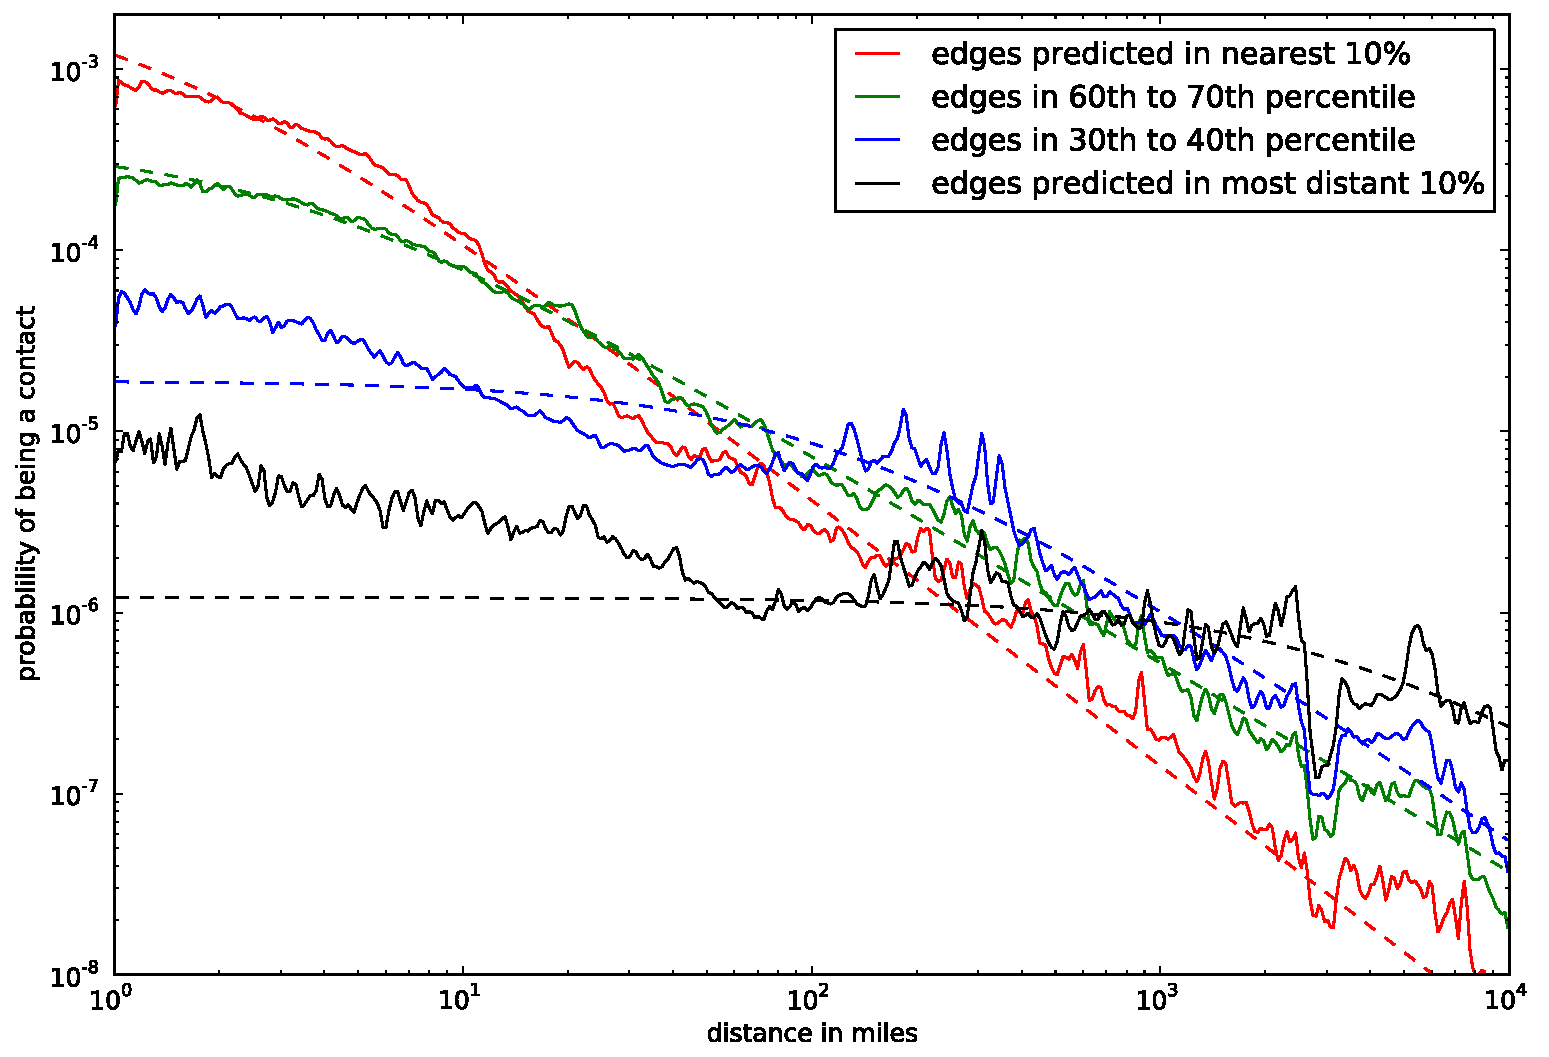
\includegraphics[width=\linewidth]{figures/near_prob_fit.pdf}
\caption{
After splitting edges into groups based on their predicted distance, each group
was fit to a curve. Here are four of the ten curves and their curves of best
fit. The other six curves of best fit are shown as faint dotted lines. The
decision tree does a reasonable job of separating the best edges from the worst
edges.
}
\label{fig:NearProbFit}
\end{figure}

We choose to use only 10 quantiles.
%
\jam{Why 10? too few - not enough data, too many, little benefit, 10 is easy to
visualize}
%
This gave us 10 different curves for the probability that a certain type of
contact exists between a pair of users.
%
Four of the ten curves from one of the five evaluation groups and their lines
of best fit are shown in Figure~\ref{fig:NearProbFit}.
%
The best contacts are orders of magnitude more
likely to live near a target user than the worst contacts.
%
If the predictions from the tree regressor were ignored, and users were placed
into one group instead of ten equal groups, this would reduce to the model
for friendship and distance presented in \cite{backstrom2010find}.


\begin{figure}[tbh]
\centering
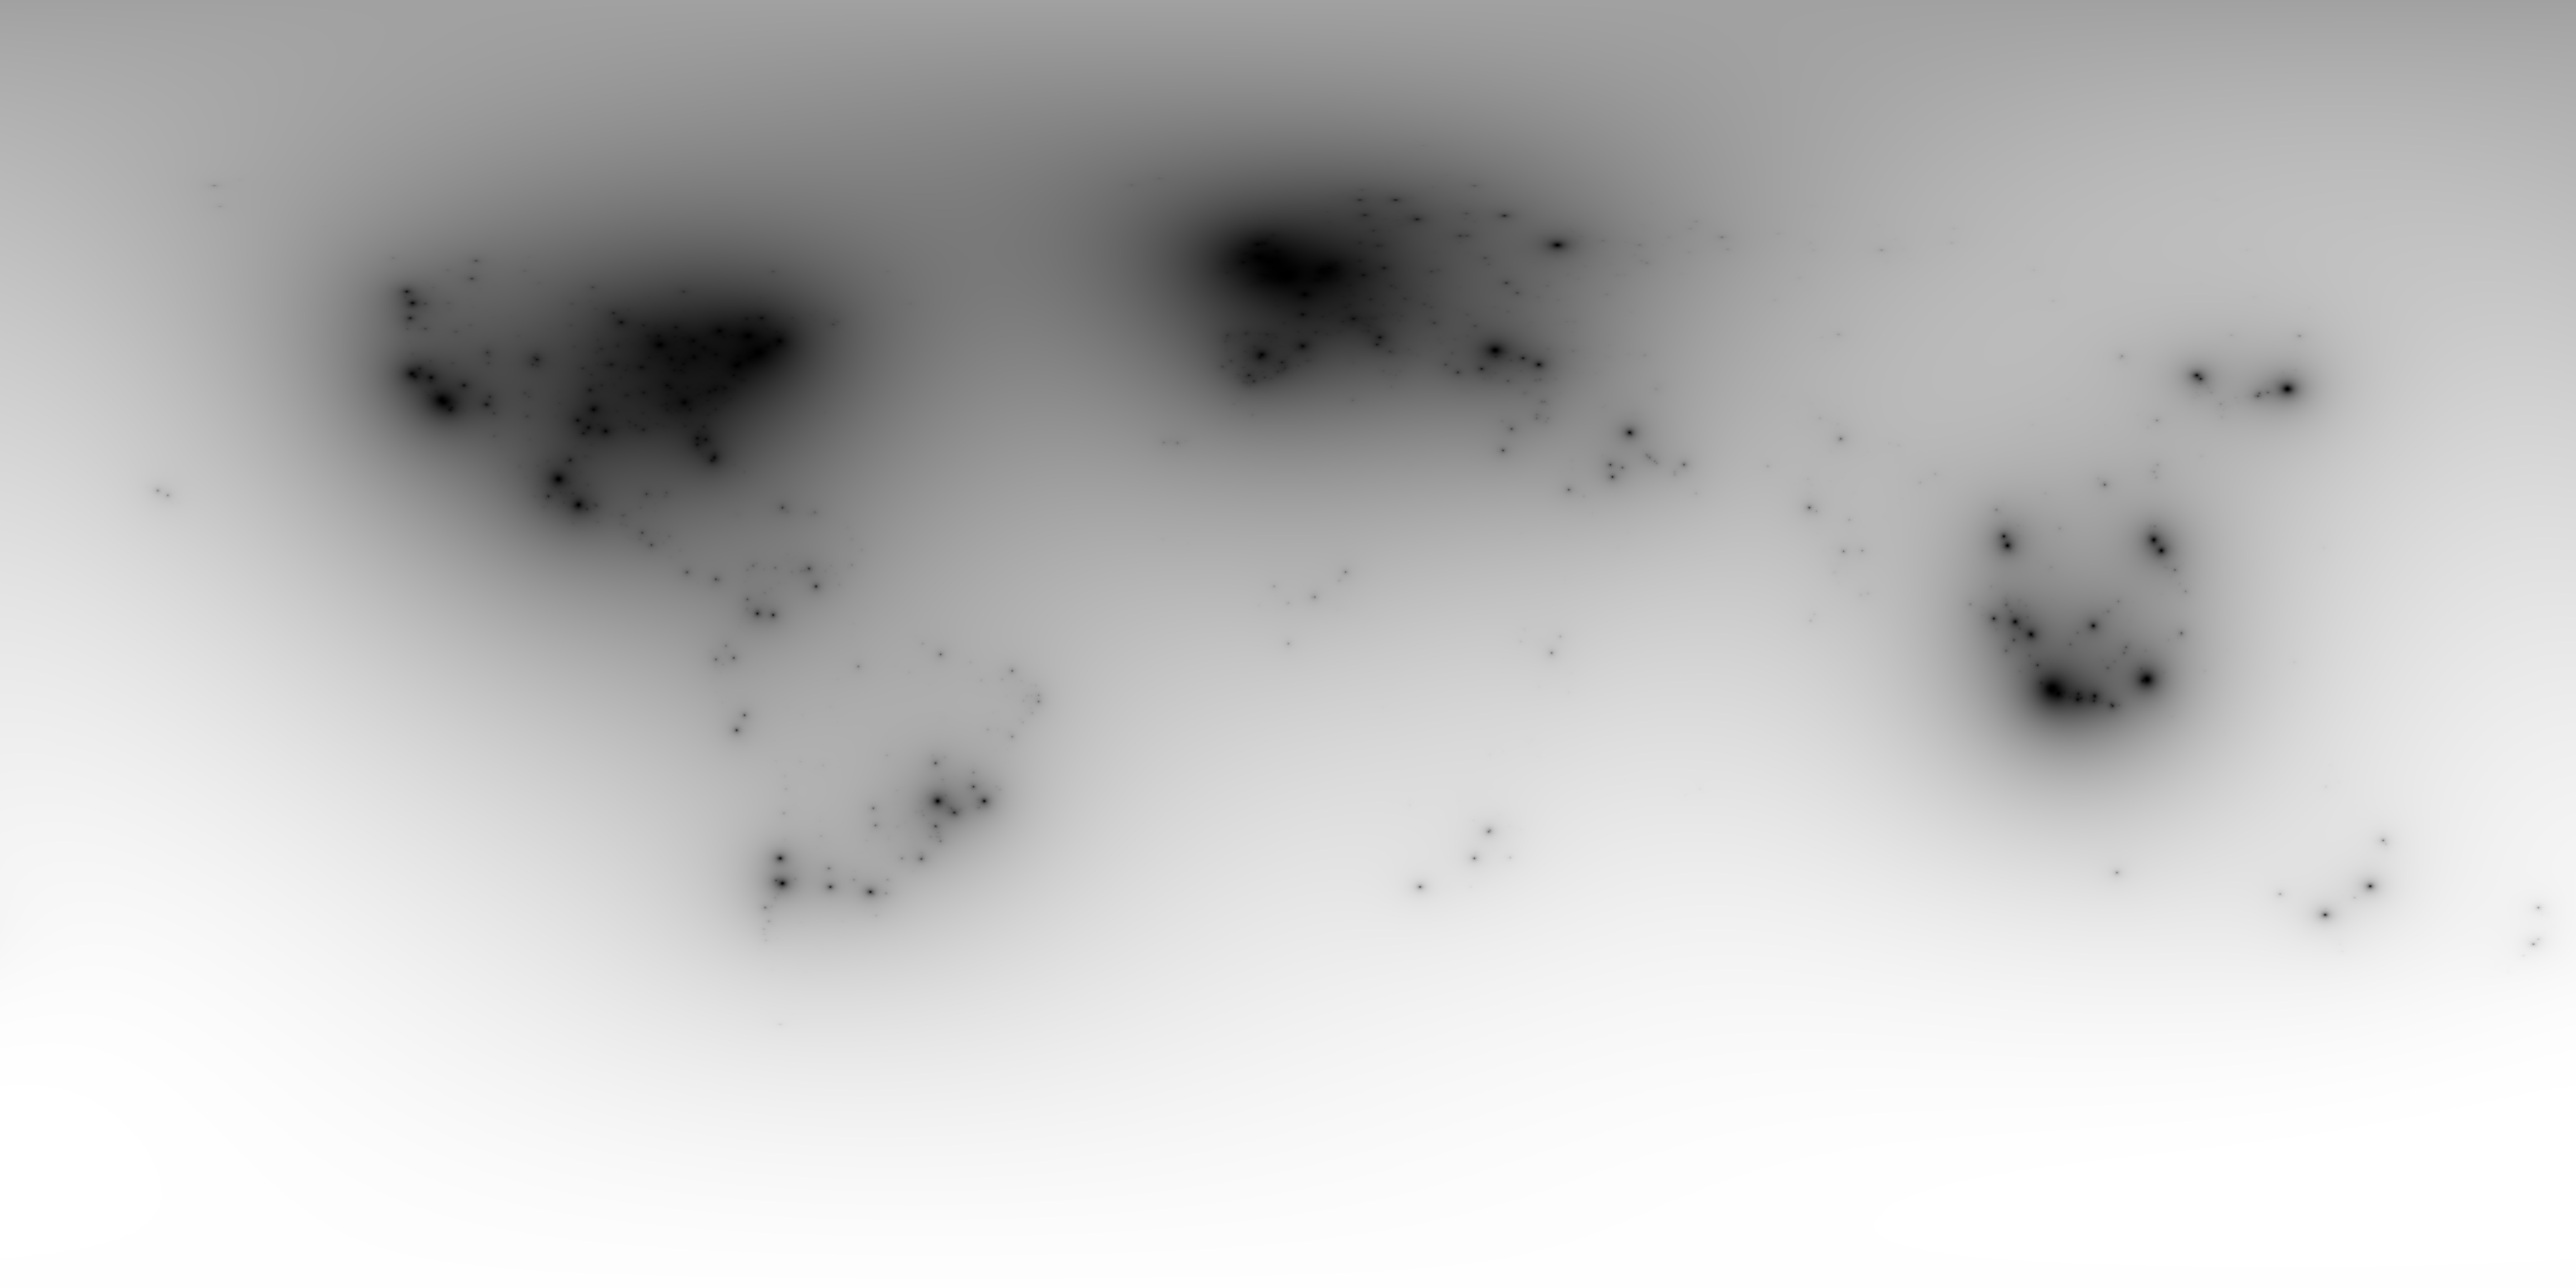
\includegraphics[width=\linewidth]{figures/stranger_mat.png}
\caption{
    This is the probability that a user lives at a location based on the people
    who they have no contact with. Dark areas have lower probability, and light
    areas have a higher probability.
}
\label{fig:StrangerMat}
\end{figure}


\section{Location Prediction System}
We used this model to improve a maximum-likelihood estimator proposed by
Backstrom et al. in \cite{backstrom2010find}.
%
The predictor they propose expressed in our notation is
\[
    \Backstrom(l,L^c) = 
        \prod_{l^c \in L^c} {\p(|l-l^c|) \over 1-\p(l-l^c) }
        \prod_{l^s \in L^s} 1-\p(|l-l^s|)
\]
where $L^c$ is the set of locations of a user's contacts, $L^s$ is the set
of all strangers' locations, and $\p$ is the probabilty of friendship given
distance.

The last product in that formula is only a function of the location $l^c_i$ and
the locations of the strangers; it does not depend on any other information
about the target user's contacts.
%
As suggested in \cite{backstrom2010find}, this can be pre-computed for every
location.
%
For convienience, we refer to this as $\pStrangers$:
\[
    \pStrangers(l) = \prod_{l^s \in L^s}1-p(|l-l^s|)
\]
Figure~\ref{fig:StrangerMat} shows $\pStrangers$ for every location on earth.
%
\jam{Do we even need to show this graph? It's not new research, but I think it
does help the reader understand pStrangers.}
%
Major cities have the lowest probability for $\pStrangers$.
%
It may seem counter-intuitive that areas with low population density have a
higher probability, but consider this example: if someone has ten friends in
New York City and ten friends in a small town in upstate New York, they are
more likely to live in the small town, and just happen to know people in the
big city.

We propose improving their system by adding in information from the decision
tree.
%
We do this by replacing the probability of being a contact based purely on
distance ($p$) to the probability we found in the previous section
($pContact$).
%
We now have a formula for predicting the best location given $L$, the set of
locations of the contacts, and $P$, the set of predicted distances to the same
contacts:
\[
    \FriendLoc(l,L,P) =
        \left(
            \prod_{l^c_k \in L,p_k \in P}
            {\pContact(\quantile(p_k),|l-l^c_k|) \over (1-p(|l-l^c_k|))}
        \right)
        \pStrangers(l)
\]

Algorithm~\ref{alg:friendloc} shows all the pieces from this section and the
previous section tied together.

\begin{algorithm}
  %\label{alg:friendloc}
  \caption{FriendlyLocation \label{alg:friendloc}}
  \begin{algorithmic}[0]
  \Input{The contacts $contacts$}
  \Output{The predicted location}
  \State locations = list()
  \State predictedDists = list()
  \ForEach{contact \textbf{in} contacts}
      \If{contact.location \textbf{is} None}
        \State \Continue
      \EndIf
      \State locations.append(contact.location)
      \State dist = regressionTree.predict(contact.features)
      \State predictedDists.append(dist)
  \EndFor
  \State best = argmax(FriendLoc(locations,predictedDists))
  \State \Return locations[best]
  \end{algorithmic}
\end{algorithm}

\jam{locations of contacts are not independent as seen in~\ref{sec:closer}, but
this formula really assumes they are. Where do we want to talk about this?}

